
%(BEGIN_QUESTION)
% Copyright 2008, Tony R. Kuphaldt, released under the Creative Commons Attribution License (v 1.0)
% This means you may do almost anything with this work of mine, so long as you give me proper credit

A technician is troubleshooting a faulty optically-isolated TRIAC power switching circuit.  The solenoid valve is supposed to open up and pass liquid through it whenever the pushbutton switch is pressed, but it remains shut no matter what state the switch is in:

$$\includegraphics[width=15.5cm]{i03178x01.eps}$$

Leaving the switch in its normal (``unpressed'') position, the technician measures 120 volts AC between test points TP5 and TP6, and 9 volts DC (normal for the battery) between test points TP1 and TP3.  Based on these voltage measurements, identify two possible faults (either one of which could account for the problem and all measured values in this circuit), and also identify two circuit elements that could not possibly be to blame (i.e. two things that you know {\it must} be functioning properly, no matter what else may be faulted).  The circuit elements you identify as either possibly faulted or properly functioning can be wires, traces, and connections as well as components.  Be as specific as you can in your answers, identifying both the circuit element and the type of fault.

\begin{itemize}
\item{} Circuit elements that are possibly faulted
\item{1.} 
\item{2.} 
\end{itemize}

\begin{itemize}
\item{} Circuit elements that must be functioning properly
\item{1.} 
\item{2.} 
\end{itemize}

\vfil 

\underbar{file i03178}
\eject
%(END_QUESTION)





%(BEGIN_ANSWER)

This is a graded question -- no answers or hints given!

%(END_ANSWER)





%(BEGIN_NOTES)

\begin{itemize}
\item{} Circuit elements that are possibly faulted
\item{1.} open TRIAC 
\item{2.} open LED 
\item{3.} open switch
\end{itemize}

\begin{itemize}
\item{} Circuit elements that must be functioning properly
\item{1.} 9 volt battery
\item{2.} AC power source
\item{3.} Good connection between battery (+) and TP1
\item{4.} Good connection between battery ($-$) and TP3
\end{itemize}

%INDEX% Troubleshooting review: electric circuits

%(END_NOTES)


